\chapter{Растяжка воображения}


\setlength{\epigraphwidth}{.80\textwidth}
\epigraph{Не стоит доверять глазам, когда воображение напряжено.
}{--- Марк Твен (1835---1910), Янки при дворе короля Артура}

Следующие головоломки потребуют от вас разработки \emph{плана},
и иногда придётся напрячь воображение!

\subsection*{Любовь в Клептопии}

Ян и Мария влюбились (по интернету), и Ян хочет послать ей по почте кольцо.
Но они живут в Клептопии, стране где все, что отправляется по почте, будет неминуемо украдено, если только оно не отправлено в запертом ящике.
У Яна и Марии много замков, но ни у кого из них нет ключа к другому.
Как безопасно переслать кольцо?

\subsection*{Черви и вода}

Лори хочет чтоб черви перестали забираются к ней на кровать.
Для этого она поставила ножки кровати в вёдра с водой;
поскольку черви не умеют плавать, они не могут добраться до кровати по полу.
Однако теперь они ползут вверх по стенам и по потолку, и падают на кровать сверху.
Фу!

Как защититься от червей?

\parit{Комментарий:}
Можно попробовать соорудить навесную конструкцию над кроватью.
Для того чтобы предотвратить падение червей на навес и их длалнейшее проползание по навесу и падение на кровать, возможно, стоит сделать жёлоб вокруг навеса и наполнить его водой.
Но ведь тогда черви смогут упасть на край желоба.
Хм...

\subsection*{Инспектор страусиных яиц}

В преддверии рекламной кампании страусиной ферме нужно проверить свои яйца на прочность.
В мировой практике, прочность определяют по самому высокому этажу в Эмпайр-стейт-билдинге с которого можно сбросить яйцо так чтоб оно не разбилось.

Официальный инспектор фирмы, Оскар, понимает, что если он возьмёт с собой в Нью-Йорк только одно яйцо,
то для определения прочности придётся (возможно) бросить его с \emph{каждого} из 102 этажей, начиная с первого.
А что если он возьмёт \emph{два} яйца?
Сколько бросков ему потребуется в худшем случае?

\subsection*{Опасная картина}

Требуется повесить картину на шнур прикреплённый к раме.
Если это сделать как обычно, перекинув нить через два гвоздя как показано на рисунке, и один из гвоздей выскочит, то картина останется висеть на другом гвозде (хотя и накренится).

Можно ли повесить картину так, чтобы она упала, если выскочит любой из двух гвоздей?

\begin{figure}[h!]
\centering
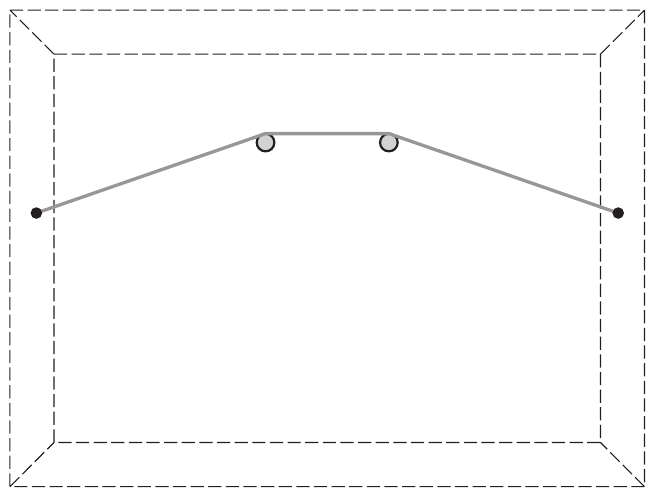
\includegraphics[scale=0.5]{pics/kartina1}
\caption{Эта картина останется висеть если выскочит один гвоздь.}
\end{figure}

\subsection*{Дефективный кодовый замок}

Кодовый замок имеет три диска, с положениями пронумерованными от 1 до 8.
У замка есть дефект, чтобы его открыть, достаточно правильно выставить только два числа.
Какое минимальное число (трёхзначных) комбинаций достаточно проверить, чтобы точно открыть замок?

\parit{Комментарий:}
Есть много способов проделать это $64$-я тестовыми комбинациями, например, можно перебрать все возможные варианты первых двух дисков, или проверить все комбинации, сумма значений которых кратна 8.
Однако каждая тройная комбинация охватывает $22$ возможных случая, а всего комбинаций $8^3 = 512$. 
Поэтому в теории может хватить $\lceil 512/22 \rceil = 24$ тестовых комбинаций.
То есть истина где-то между $24$ и $64$; вопрос где?

\subsection*{Альтернативные кости}

Можете ли сделать два игральных кубика так, чтобы их суммы вели себя так же, как пара обычных кубиков?
То есть должно быть два способа выбросить 3, шесть способов выбросить 7, один способ выбросить 12 и так далее. Кубики должны иметь по шесть граней, и на каждой грани должно быть указано положительное целое число.

\subsection*{Совпадение монет}

Сонни и Шер играют в следующую игру.
В каждом раунде бросается честная монета.
Перед бросанием монеты Сонни и Шер одновременно объявляют свои предположения о результате броска монеты.
Они выигрывают раунд, если оба угадали правильно.
Цель --- максимизировать долю выигранных раундов, когда игра идёт в течение многих раундов.

Пока что ответ очевиден --- 50\%: Сонни и Шер договариваются о последовательности предположений (например, они решают всегда говорить «орёл»).
Очевидно, что лучшего добиться нельзя.

Однако перед началом игры игрокам сообщается, что прямо перед первым броском Шер получит результаты всех бросков монеты заранее!
Теперь у неё есть возможность обсудить стратегию с Сонни, но как только она получит информацию о бросках монеты, возможности передачи информацию больше не будет.
Возожно ли дотянуть долю выигрышей скажем до 70\%?

\subsection*{Имена в коробках}

Имена 100 заключённых помещают в 100 деревянных коробок, по одному имени в коробке;
коробки расставляются в комнате на столе.
Поочерёдно заключённых проводят в комнату;
каждому позволяется заглянуть не более чем в 50 коробок,
затем он должен покинуть комнату, оставив её в точно том же состоянии как и до прихода,
дальнейшее общение с остальными невозможно.

У заключённых есть возможность спланировать свою стратегию заранее, и им это понадобится --- если хотя бы один заключённый не найдёт своё имя, то казнят всех.
Найдите стратегию, вероятность успеха которой превысит 30\%.

\parit{Комментарий:} Если каждый заключённый откроет случайный набор из 50 коробок, то вероятность выжить составлит незавидные $(\tfrac12)^{100}\approx 0{,}0000000000000000000000000000008$.
Но можно поступить и хуже --- если все откроют одни и те же 50 коробок, то их шансы упадут до нуля.
Но ведь тридцать процентов кажутся абсолютно недостижимыми...
Очень хорошо --- вы правильно поняли задачу!
